\chapter{Realizacja projektu}


\section{Wykorzystane technologie}

\subsection{Język programowania Python}

Kod projektu został napisany w języku Python. Wybór tego języka był spowodowany szeroką dostępnością bibliotek i
narzędzi wspomagających uczenie maszynowe. W szczególności należy zwrócić uwagę na biblioteki \textit{Tensorflow} oraz \textit{PyTorch}.
Są to dwie najpopularniejsze biblioteki do operowania na tensorach (tensor to uogólnienie macierzy na wiele wymiarów).
Obie pozwalają na przyśpieszanie obliczeń z użyciem zewnętrznych akceleratorów takich jak np. karty graficzne.

Podczas prac badawczych, wykorzystana wersja Pythona to \textit{3.12.0}.

\subsection{Biblioteka PyTorch}

Biblioteka PyTorch jest obecnie najpopularniejszą biblioteką uczenia maszynowego.
Pozwala ona projektować obliczenia w formie modułów i posiada silnik automatycznego różniczkowania grafu obliczeniowego (z ang. \textit{autograd}).
Owy silnik jest kluczowy z perspektywy trenowania sieci neuronowych, ponieważ jest w stanie optymalizować parametry modelu.
Warto zwrócić uwagę na to, że PyTorch stawia nacisk na przejrzystość obliczeń - dla porównania operacje w Tensorflow są nierzadko
ukryte pod gotowymi funkcjami (zob. listing \ref{lst:tensorflow_sample} i \ref{lst:pytorch_sample})

\begin{lstlisting}[language=ipython,caption={Przykładowa sieć neuronowa w Tensorflow},label={lst:tensorflow_sample}]
tensorflow_model = tf.keras.Sequential([
    tf.keras.layers.Flatten(input_shape=(28, 28)),
    tf.keras.layers.Dense(128, activation='relu'),
    tf.keras.layers.Dense(10, activation='softmax')
])

tensorflow_model.compile() # Brak doglebnej kontroli nad przeplywem obliczen
\end{lstlisting}


\begin{lstlisting}[language=ipython,caption={Przykładowa sieć neuronowa w PyTorch},label={lst:pytorch_sample}]
class PyTorchNetwork(nn.Module):
    def __init__(self):
        super(Net, self).__init__()
        self.flatten = nn.Flatten()
        self.fc1 = nn.Linear(28 * 28, 128)
        self.relu = nn.ReLU()
        self.fc2 = nn.Linear(128, 10)

    def forward(self, x): # Dokladna kontrola nad przeplywem obliczen
        x = self.flatten(x)
        x = self.fc1(x)
        x = self.relu(x)
        x = self.fc2(x)
        return x
\end{lstlisting}

PyTorch oferuje również zestaw narzędzi do przetwarzania danych, dostarcza również gotowe, pretrenowane modele dla najpopularniejszych architektur.
Przykładami są pakiety \textit{torchvision} lub \textit{torch.utils}. Cała biblioteka jest w stanie wykorzystywać karty graficzne (z ang. \textit{graphical processing unit, GPU}) do przyspieszania obliczeń.

\subsection{Biblioteka OpenCV}

Biblioteka OpenCV \cite{opencv} dostarcza implementacje wielu konwencjonalnych algorytmów wizji komputerowej.
OpenCV eksponuje interfejs programistyczny, dzięki któremu programista Pythona może komunikować się z implementacją algorytmów w C++.
To zapewnia szybkość wykonywania obliczeń, jednocześnie nie wymuszając na programiście pisania kodu w C++. Przykład wykorzystania biblioteki OpenCV widoczny jest na listingu \ref{lst:opencv_sample}
- kod wylicza momenty Hu.

OpenCV w niniejszej pracy jest wykorzystywane do automatycznej ekstrakcji kwadratów z komórkami na podstawie dużego zdjęcia spod mikroskopu.
Więcej informacji na ten temat w rozdziale \ref{sec:automatyczny-licznik-limfoblastow}.

\begin{lstlisting}[language=ipython,caption={Obliczenie momentów Hu z użyciem OpenCV}, label={lst:opencv_sample}]
import cv2

image = cv2.imread('obraz.jpg', 0)  # 0 oznacza wczytanie obrazu w odcieniach szarosci

hu_moments = cv2.HuMoments(cv2.moments(image)).flatten()

print("Momenty Hu:")
for i in range(0, 7):
    print(f"Moment {i+1}: {hu_moments[i]}")
\end{lstlisting}

\subsection{Inne narzędzia}

Kod źródłowy projektu był przechowywany w repozytorium na platformie GitHub (dostępny pod adresem \url{https://github.com/matisiekpl/thesis}).
Wykresy były generowane za pomocą biblioteki \textit{matplotlib} \cite{matplotlib},
a metryki liczone z użyciem funkcji pakietu \textit{scikit-learn} \cite{scikit_learn}.

\subsection{Sprzęt}

Do prac badawczych został użyty Apple Macbook Pro 2020 (M1/16GB pamięci). Trenowanie sieci odbywało się na platformie \textit{kaggle.com}, która oferuje bezpłatne 30 godzin obliczeń co miesiąc z kartą graficzną \textit{NVIDIA P100}.


\section{Zbiór danych}

Wykorzystany w projekcie zbiór danych to kolekcja 170 tysięcy zdjęć komórek z rozmazów szpiku kostnego.
Zdjęcia mają nadane etykiety przez diagnostów i przedstawiają różne komórki widziane pod mikroskopem.
Próbki szpiku kostnego pochodzą z biopsji 945 pacjentów z Monachijskiego Labolatorium Białaczek (\textit{MLL Münchner Leukämielabor} \cite{mll}).
Akwizycja obrazu polegała na wykonaniu zdjęcia mikroskopią Brightfield'a z 40-krotnym powiększeniem.
Producentem mikroskopu było przedsiębiorstwo Fraunhofer IIS.

Komórki były barwione metodą Maya-Grünwalda-Giemsa. Zbiór danych zawiera 21 klas. Tabela klas jest widoczna w tabeli \ref{tab:images_count},
a wizualizacja ilościowa na rys. \ref{fig:images_count_vis}

\begin{table}
    \begin{center}
        \caption{Klasy obrazów w zbiorze danych}
        \label{tab:images_count}
        \begin{tabular}{|l|l|l|}
            \hline
            Klasa & Nazwa & Liczba obrazów \\
            \hline
            NGS & Segmentowany neutrofil & 29001 \\
            \hline
            EBO & Erytroblast & 27396 \\
            \hline
            LYT & Limfocyt & 26242 \\
            \hline
            ART & Artefakt & 19630 \\
            \hline
            PMO & Promielocyt & 11994 \\
            \hline
            BLA & Blast & 11973 \\
            \hline
            NGB & Krwinka biała pałeczkowata & 9968 \\
            \hline
            PLM & Komórka plazmatyczna & 7630 \\
            \hline
            MYB & Mielocyt & 6558 \\
            \hline
            EOS & Eozynofil & 5883 \\
            \hline
            MON & Monocyte & 4040 \\
            \hline
            NIF & Brak rozpoznania & 3538 \\
            \hline
            MMZ & Metamielocyt & 3055 \\
            \hline
            PEB & Proerytroblast & 2740 \\
            \hline
            BAS & Bazofil & 441 \\
            \hline
            HAC & Włochata komórka & 409 \\
            \hline
            OTH & Inna komórka & 294 \\
            \hline
            LYI & Niedojrzały limfocyt & 65 \\
            \hline
            FGC & Fagocyt & 47 \\
            \hline
            KSC & Cienie komórkowe & 42 \\
            \hline
            ABE & Nieprawidłowy eozynofil & 8 \\
            \hline
        \end{tabular}
    \end{center}
\end{table}

\begin{figure}
    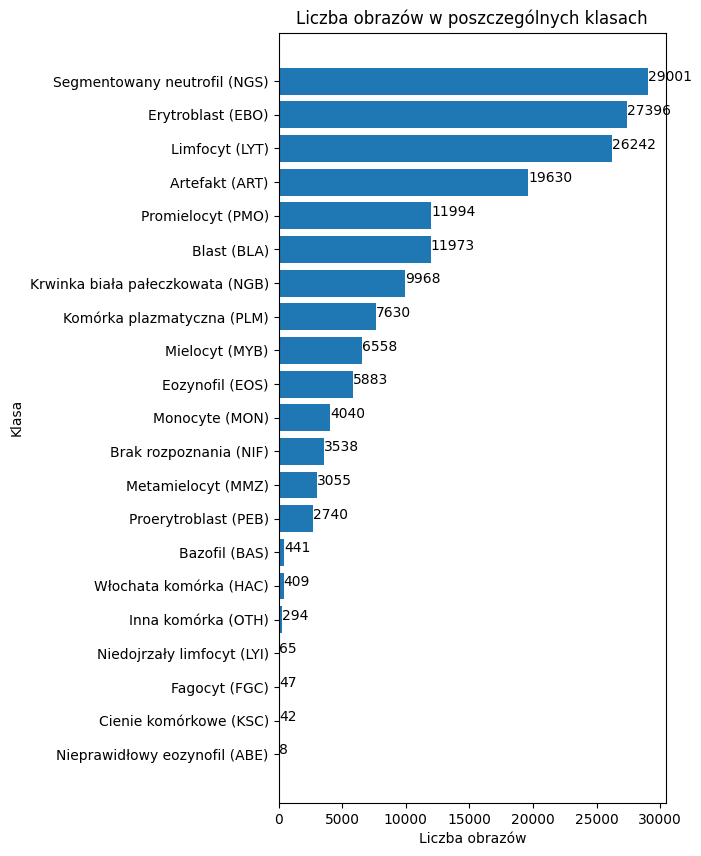
\includegraphics[width=\textwidth]{images_count}\label{fig:images_count_vis}
    \caption{Wizualizacja ilościowa rozkładu próbek w klasach w zbiorze danych}
\end{figure}

%\begin{itemize}
%    \item Nieprawidłowy eozynofil
%    \item Artefakt
%    \item Bazofil
%    \item Blast
%    \item Erytroblast
%    \item Eozynofil
%    \item Fagocyt
%    \item Włochata komórka
%    \item Cienie komórkowe
%    \item Niedojrzały limfocyt
%    \item Metamielocyt
%    \item Krwinka biała pałeczkowata
%    \item Segmentowany neutrofil
%    \item Brak rozpoznania
%    \item Inna komórka
%    \item Proerytroblast
%    \item Komórka plazmatyczna
%    \item Promielocyt
%\end{itemize}


\section{Struktura projektu}

\subsection{Przygotowanie danych}

\subsection{Trening sieci neuronowej}

\subsection{Ocena jakości modelu}


\section{Interfejs użytkownika}


\section{Automatyczny licznik limfoblastów}\label{sec:automatyczny-licznik-limfoblastow}

